\subsection{Agentes Racionais}
“Mas seria possível uma maquina pensar?“ Esse foi o questionamento inicial de Turing, visando a resposta ele propôs o \textit{Imitation Game} que basicamente se consiste colocar uma pessoa (1) para conversar com um computador, esse computador poderá ser uma Inteligência Artificial ou outra pessoa (2) conversando escondida através da maquina, o objetivo é que a pessoa 1 consiga distinguir se quem esta conversando com ela é a maquina ou a pessoa 2. A proposta feita por Turing seria considerada como um \textbf{agir humanamente}, ela se baseia em criar uma maquina que reconhece a escrita, tome decisões a partir de um centro de referencias e por final seja capaz de se aprimorar diante de novos cenários. Porem, como seria desenvolvido algo de tal amplitude? A resposta é que “não seria”, questionar se uma máquina é capaz de pensar seria o mesmo que questionar se um submarino é capaz de nadar, afirmou Dijsktra, quando aponta que o termo "pensar" e "nadar" tinham suas definições restritas, entretanto, era possível realizar ações similares tão bem quanto \cite[2-3]{dijkstra898, turing1950, russell2003artificial}.

Para realizarmos as ações descritas por Turing, precisamos entender seus processamentos de forma racional e lógica afim de replica-los para a maquina. A abordagem de \textbf{agentes racionais} é uma das possibilidades a serem usadas. O termo racional significa algo baseado ou acordado com uma razão ou lógica, de outro lado, a lógica tem dois pilares: a \textbf{conversão} responsável por expressar a mesma proposição em diferentes formas e o \textbf{silogismo} responsável por localizar um termo em comum que conecte duas dessas proposições. Um agente é algo que age, ou seja, um agente racional seria quem analisa circustancias utilizando de definições lógicas e racionais a fim de interagir com algo. Isso é afirmado pela definiçao de Russel, onde um agente raciona percebe modificações no ambiente através de sensores e interage de volta com o ambiente através de atuadores, pode-se notar esse fluxo na figura \ref{fig:rational_agent_draw}. Logo, podemos afirmar, que para ser possível realizar ações racionais é necessário entender o ambiente aonde você esta e suas variáveis, alias, é necessário que esteja claro o que pode ou não ser computado, quais são as regras que podemos aplicar e principalmente como conseguimos obter algo racional em caso informações incertas. \cite[7]{frege1956thought, wooldridge1994agent, simon1955behavioral, boole1854investigation, russell2003artificial}

\begin{figure*}
    \centering
    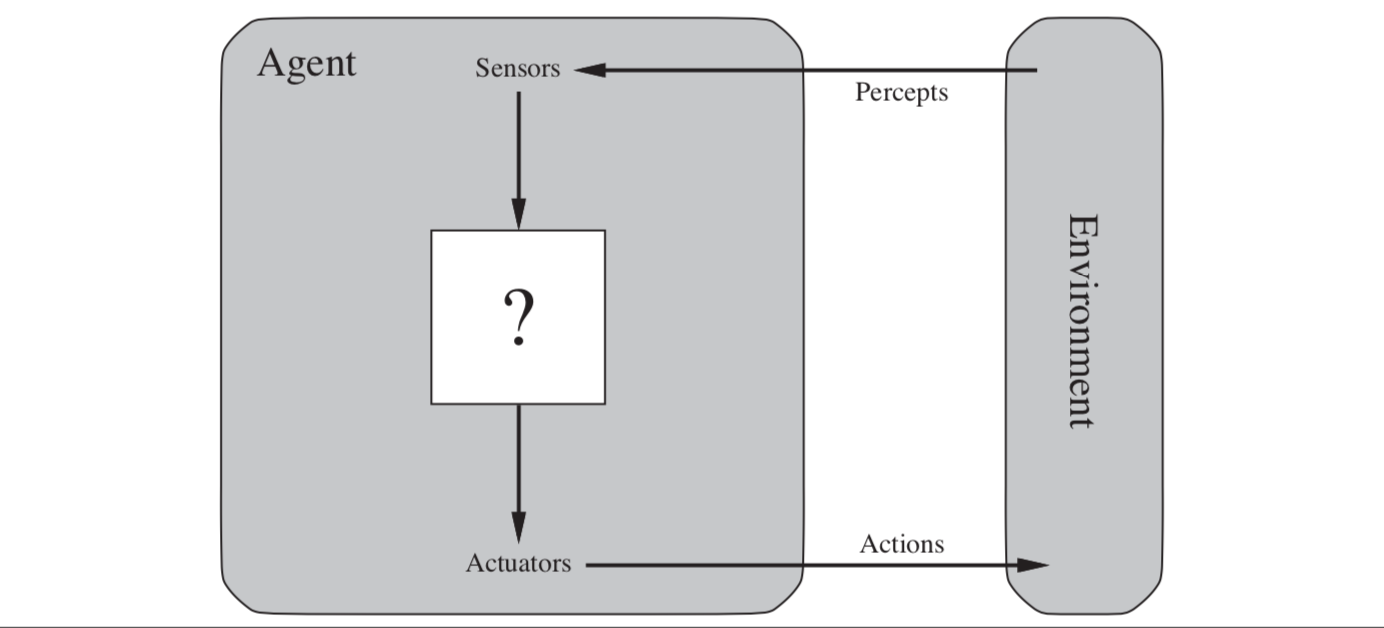
\includegraphics[width=.8\textwidth]{imagens/rational_agent_draw.png}
    \caption{Sentiment variation before and after interaction with ANY developer, in the one-hour time window.}
    \label{fig:rational_agent_draw}
\end{figure*}

Para que seja possível definir se o agente está ou não gerando os dados esperados é necessário medir sua performance, então, é necessário que analisar o ambiente gerado a partir das percepções e conferir se os dados são os esperados ou não. Em resumo o agente recebera um entrada de dados e será responsável por gerar um saída, ao longo do tempo o mesmo agente gerara múltiplas percepções e essas formarão uma sequencia de percepções \footnote{Não serão todos os modelos que seguirão a proposta sequencial, existem casos em que a linha temporal não afeta o desenvolvimento da decisões tornando-as episódicas}. Existem definições dadas aos agentes racionais, iremos definir algumas delas a seguir \cite[34-45]{russell2003artificial}:

\begin{itemize}
 \item \textbf{Totalmente, parcialmente ou não observador:} essa definição é gerada pela quantidade de fatores do ambiente que seu agente recebe, um agente que tem todas as informações do ambiente é totalmente observador enquanto um que não recebe nada, precisando assim manter alguns estados, é não observador.
 \item \textbf{Estocástico ou Determinístico:} quando é impossível determinar o próximo estado através do anterior o agente é Estocástico, caso ao contrario ele é Determinístico.
 \item \textbf{Episódicos ou Sequenciais:} já foi dito que em diversas abordagens são gerados sequencias de percepção, quando essa sequencia é alterado a partir de alguma mudança de estado chamamos o agente de sequencial, caso ao contrario o agente é Episódico.
 \item \textbf{Estáticos ou Dinâmicos} essa definição é referente ao ambiente, quando nosso ambiente não infere alterações chamamos o agente de estático, caso ao contrario Dinâmico.
 \item \textbf{Continuo ou Distinto:} Quando existem finitas possibilidades de estado pode se afirmar que o agente é Distinto, quando as possibilidades são infinitas é dado o nome de Continuo.
 \item \textbf{Conhecido ou Desconhecido:} Quando o agente necessita aprender algo e não consegue realizar a ação por si só ele é um agente desconhecido, caso ao contrário ele é conhecido.
\end{itemize}

